\subsection{\href{https://www.lacolmena.com.ar/}{La Colmena}}
   \hypertarget{subsec:colmena}
   For the well-known disc of Pilar, La Colmena, a LED ceiling was developed and manufactured using Ethernet with the sophisticated software Madrix, highlighting the photos of the installation in the figure \ref{fig:colmena} and there are also some public videos on \href \linkcolmenavideos {videos La Colmena}.
   \begin{figure}
      \begin{center}
         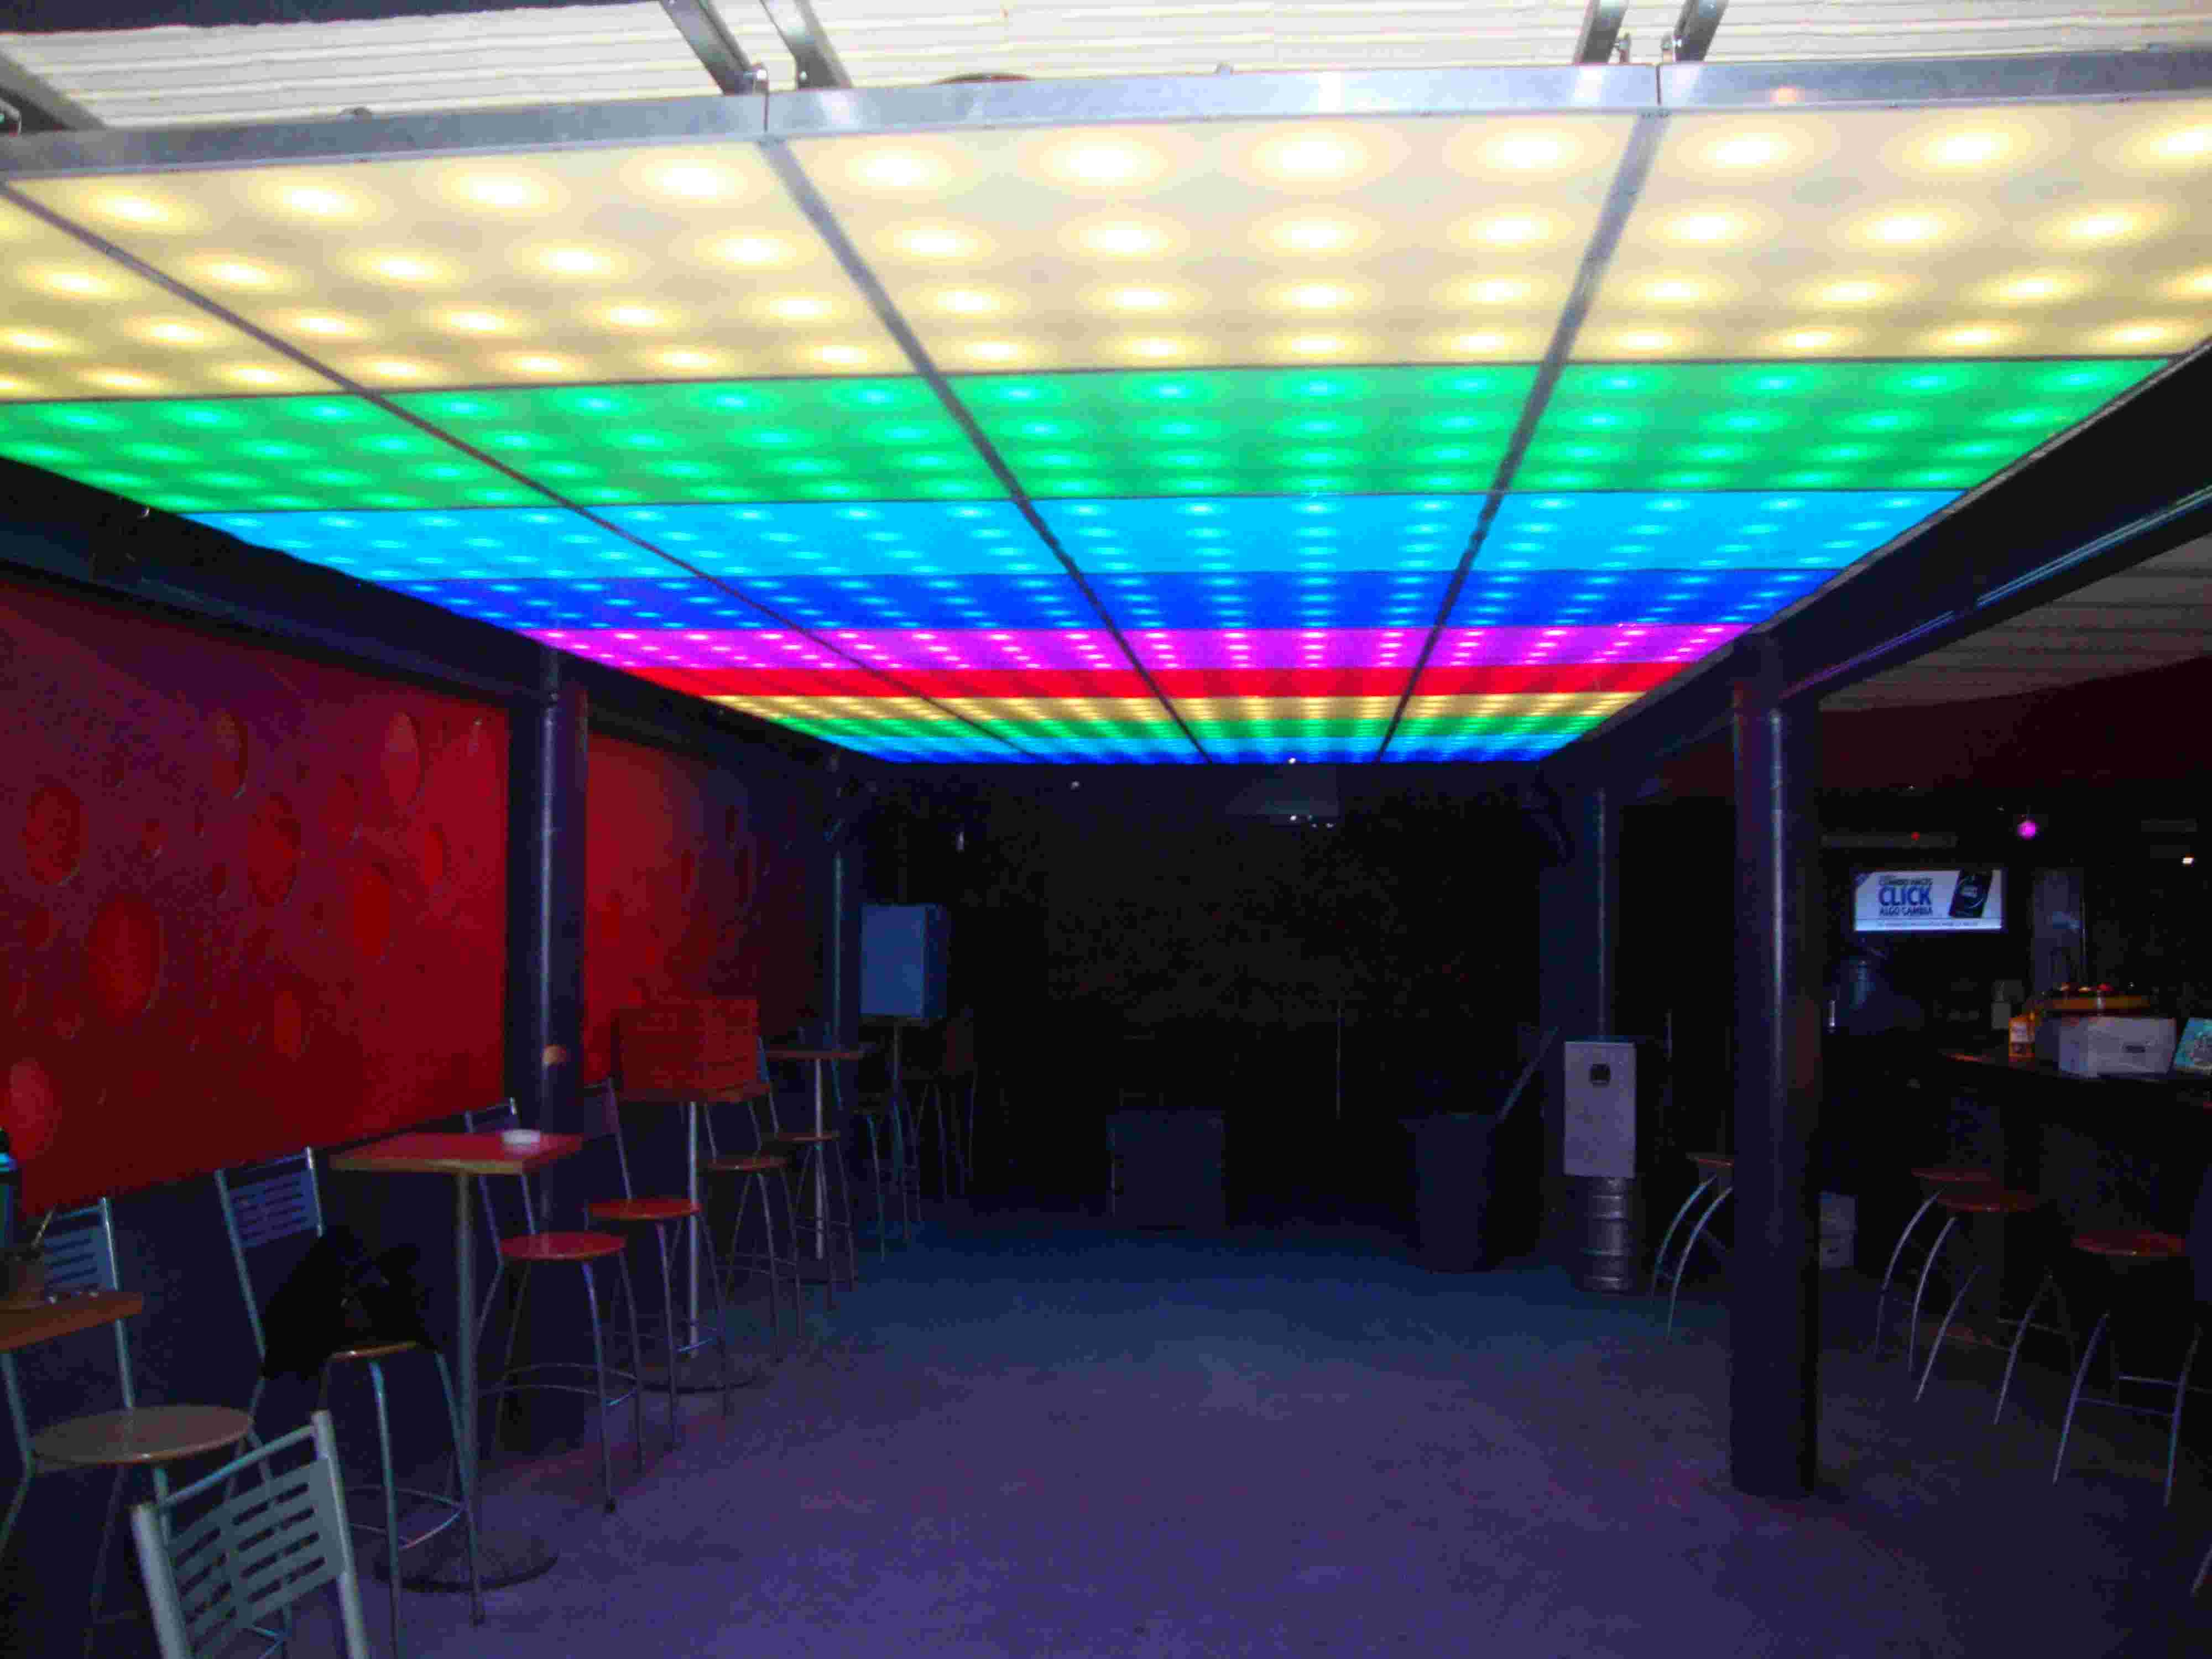
\includegraphics[width=0.24\textwidth]{colmena1.jpg}
         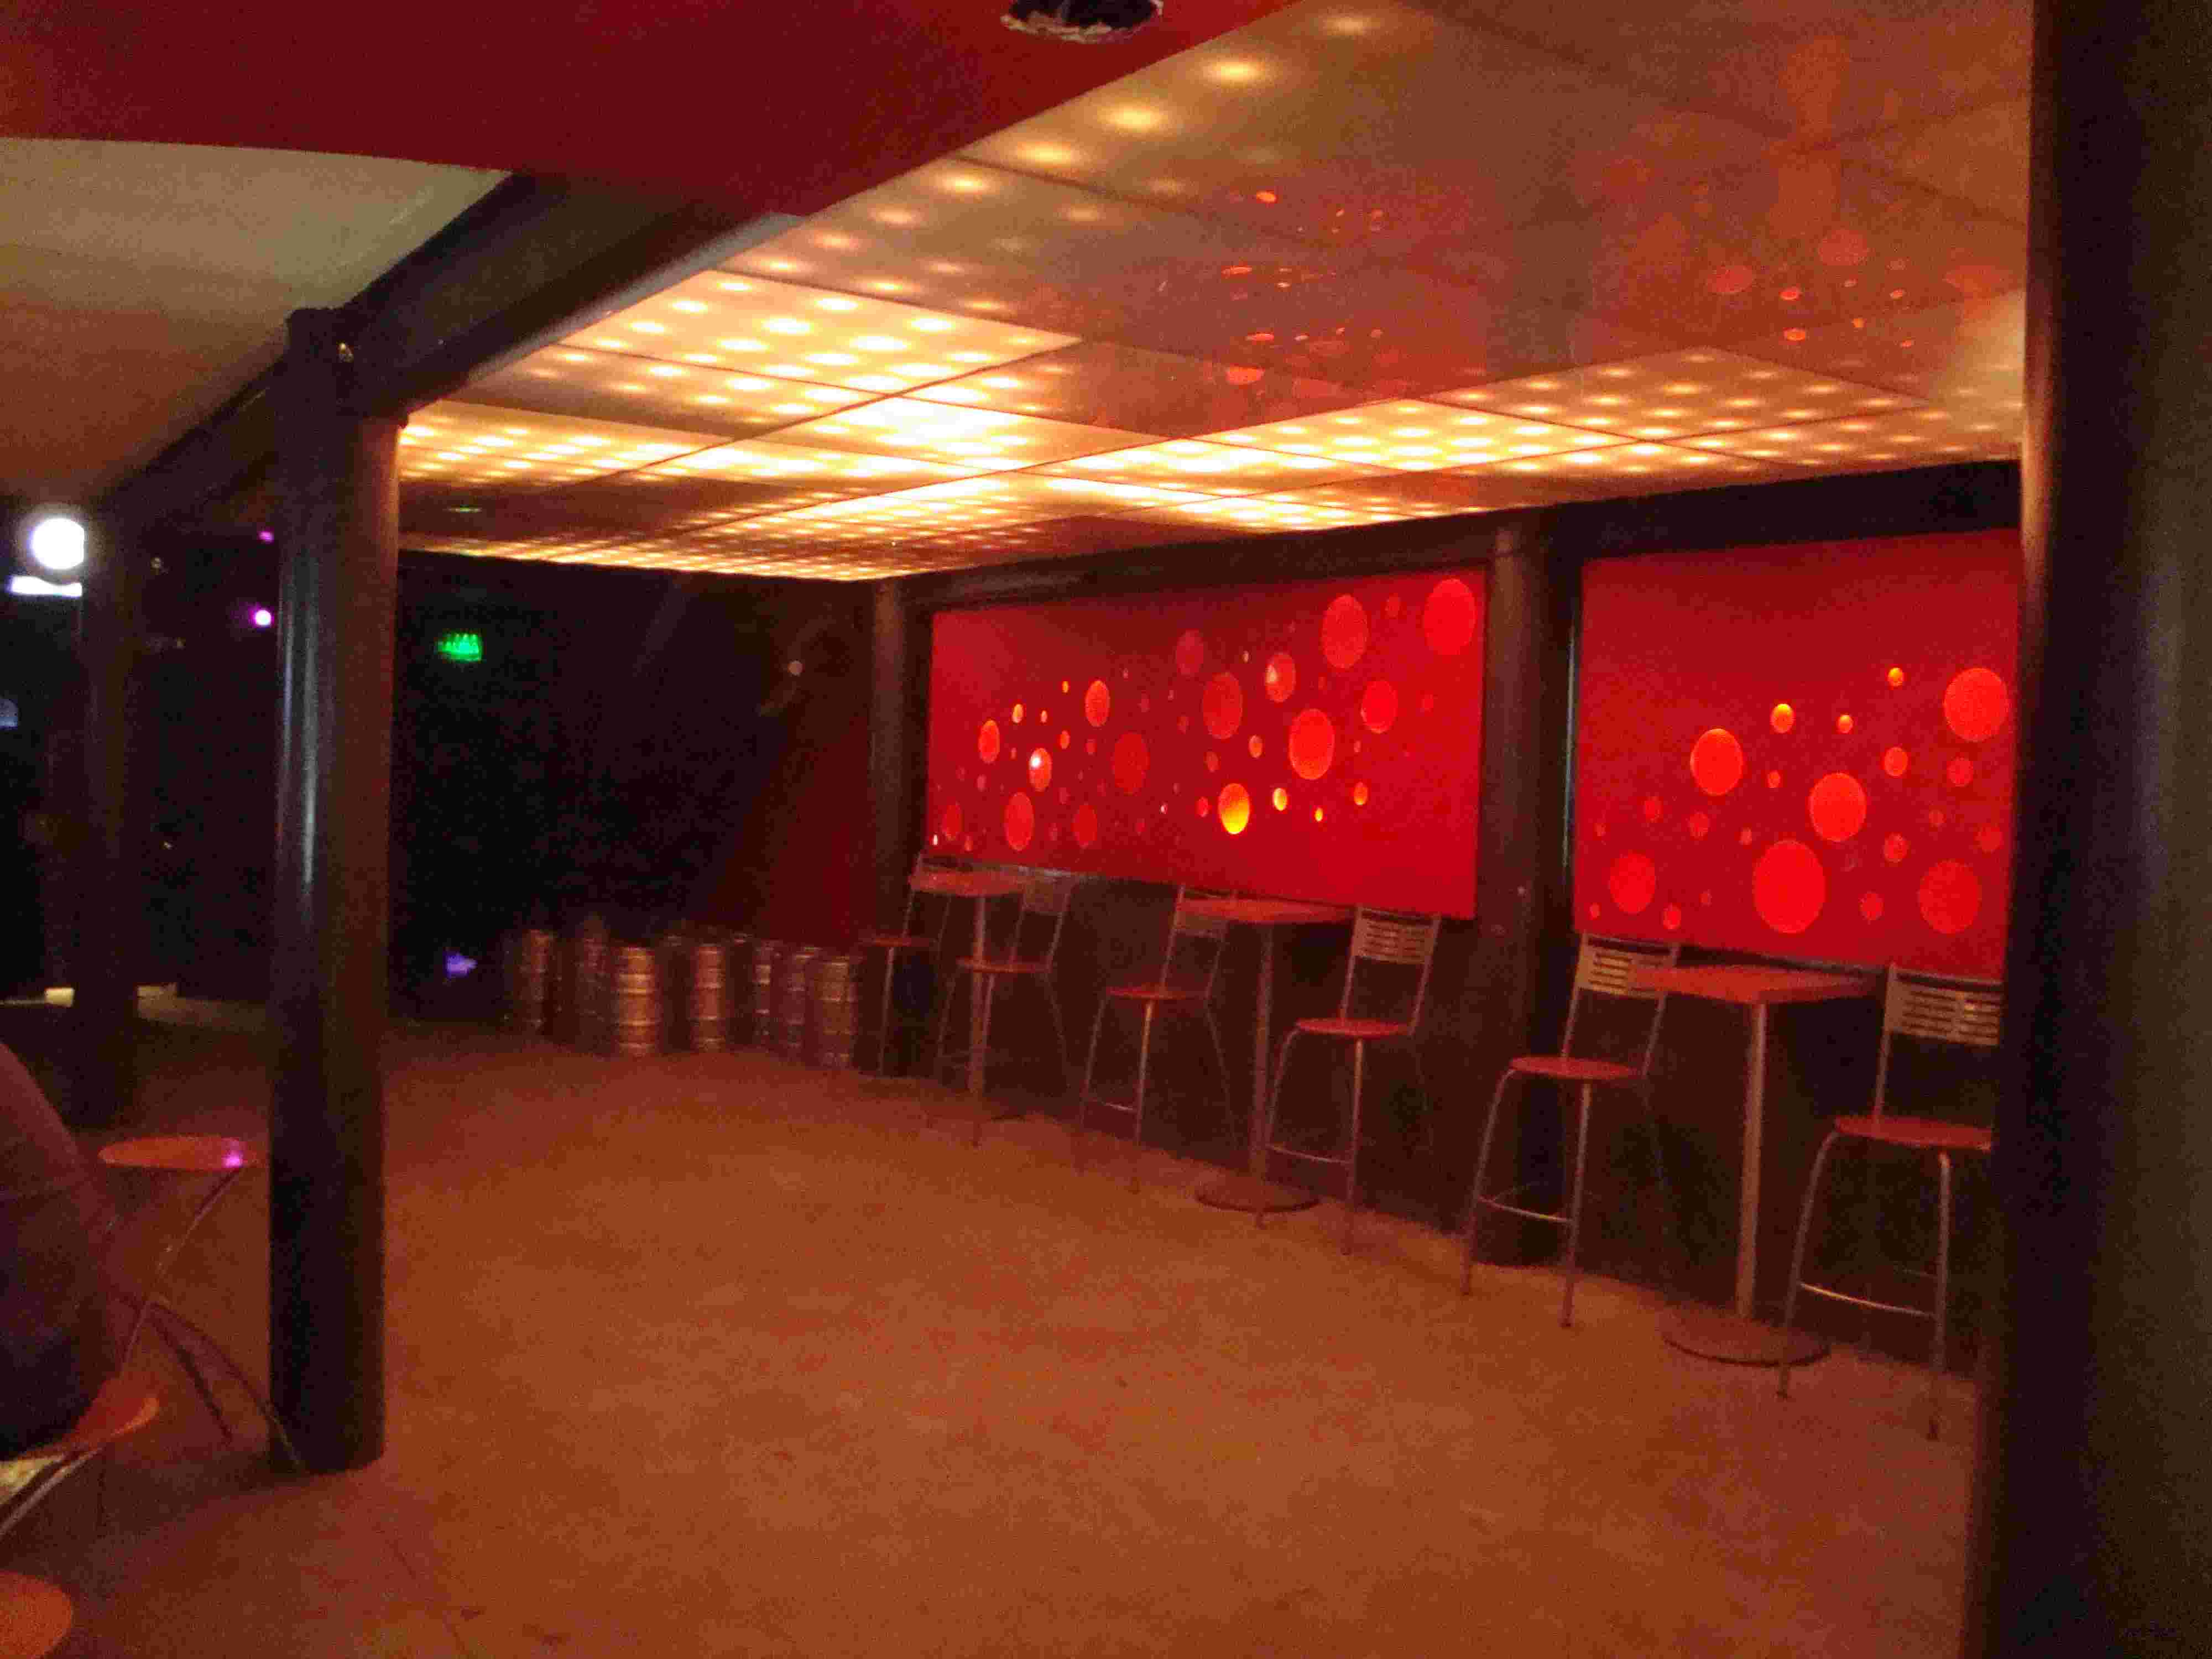
\includegraphics[width=0.24\textwidth]{colmena2.jpg}
         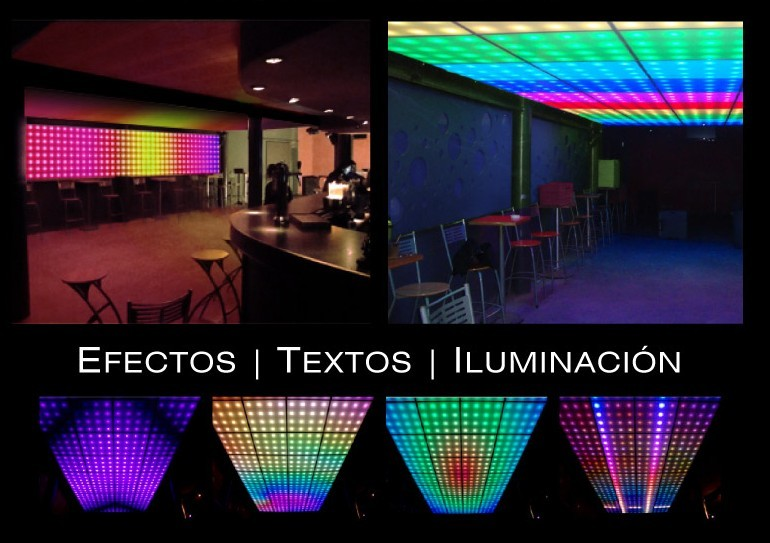
\includegraphics[width=0.24\textwidth]{colmena3.jpg}
         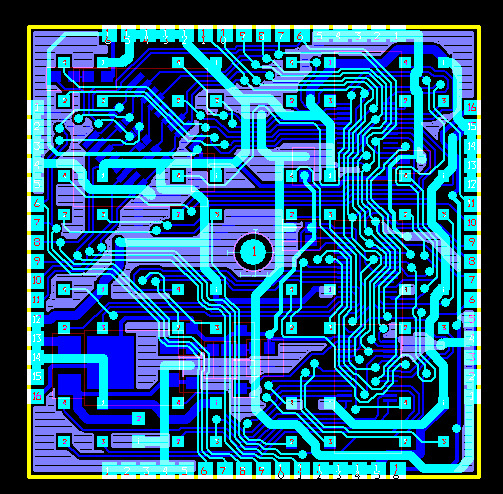
\includegraphics[width=0.24\textwidth]{colmena4.jpg}
      \end{center}
      \caption{LED display mounted on the roof of the La Colmena disc, developed, manufactured and installed.}
      \label{fig:colmena}
   \end{figure}
   \par
From this work, a product that consists of interconnected modules to form LED screens different pitch and sizes. Can you see in the pictures of the figure \ref{fig:ledcover} and you can see some videos at \href \linkledcovervideos {see videos}.
   \begin{figure}
      \begin{center}
         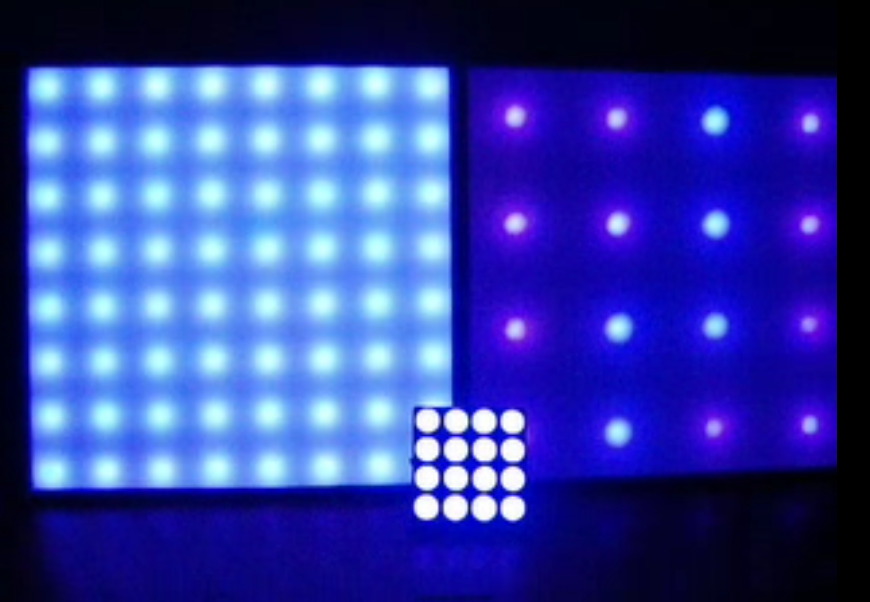
\includegraphics[width=0.24\textwidth]{ledcover1.jpg}
         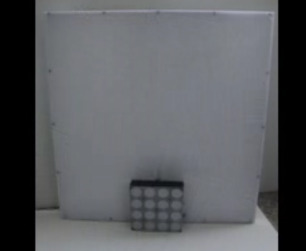
\includegraphics[width=0.24\textwidth]{ledcover2.jpg}
         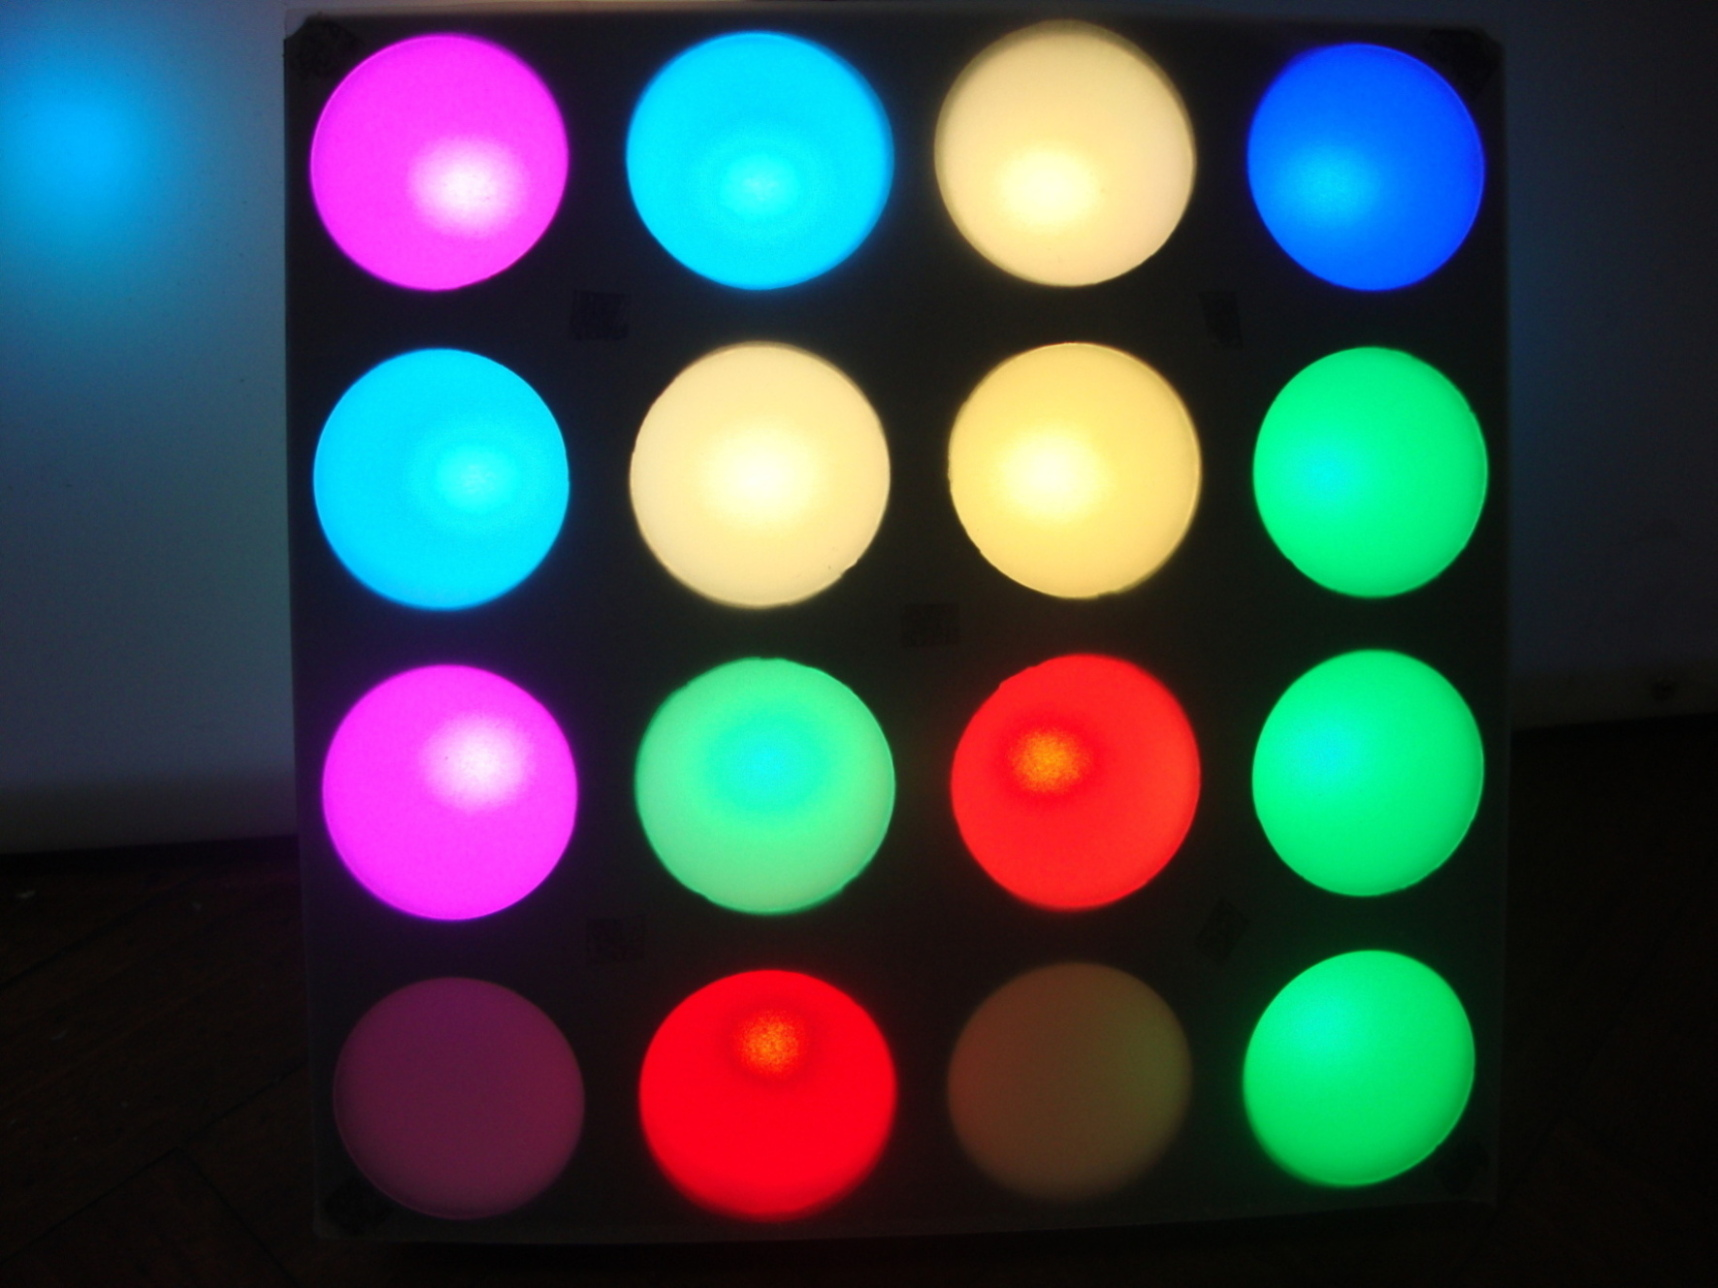
\includegraphics[width=0.24\textwidth]{ledcover3.jpg}
         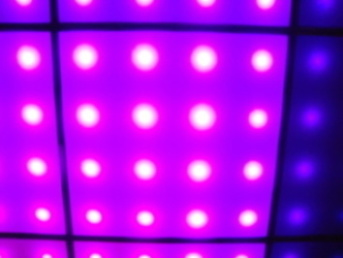
\includegraphics[width=0.24\textwidth]{ledcover4.jpg}
      \end{center}
      \caption{Modules of interconnectable LEDs to form LED screens controlled by ethernet of different pitch and sizes.}
      \label{fig:ledcover}
   \end{figure}
